\section{Numerical}

In this section, numerical experiments will be conducted to test the developed method,
and to evaluate wether it can be deployed in a real scenario.

The experiment will proceed in the following way:
in the first place, a profile for a theoretical travel time function will be defined.
This profile will need to satisfy assumptions NUMBERS\todo{Cite all the assumptions},
in order to be similar to a profile that could be found in reality.

After the function has been defined,
shapes for the distributions of the parameters \(B, \Gamma, T^*\) will be fixed,
dependant on a parameter \(\theta \in \R^d\).

Given all of this and a value \(\theta_0\) for the shape parameter \(\theta\),
a dataset of synthetic observations can be built accordingly to the model.
The dataset is constructed by sampling the parameters \(\beta, \gamma, t^*\) and explicitly minimizing the resulting cost function.
This yields a dataset for which the real value of the parameter \(\theta\),
which affects the distributions of \(B, \Gamma, T^*\), is known,
allowing the actual convergence of the estimation to be evaluated in a simple scenario,
and the behaviour of the likelihood function to be shown when the dataset is fixed.

\subsection{Choosing the parameters}

As explained above,
the first step to be done consists in choosing the travel time function and the distributions of the parameters.

\subsubsection{Travel Time Function}

The travel time function must be chosen accordingly to assumptions \todo{What assumptions?}:
it hence has to be continuous and with continuous derivative,
and its derivative upper bounded by \(1\).
Moreover, it has to satisfy assumption \todo{assumption number},
that defines when the function is concave and when convex.

A gaussian function satisfies all the assumptions,
as long as its variance is high enough.
For better capturing the expected asymmetricity for early and late arrivals,
two different variances will be considered before and after the peak.
The considered function will thus be
\begin{equation}
  \label{eq:tt_def}
  tt(t) =
  \begin{cases}
    e^{-\frac{(x - \mu)^2}{\sigma_l}} & \text{if } x \leq \mu \\
    e^{-\frac{(x - \mu)^2}{\sigma_r}} & \text{if } x > \mu
  \end{cases}
\end{equation}

The resulting function is shown in figure\todo{Put figure}.
It satisfies assumption NUMBER\todo{put number},
since
\begin{equation*}
  \lim_{t \rightarrow 0}tt'(t) = 0.
\end{equation*}
Moreover, by setting an high enough value for the parameter \(\sigma_l\),
determining the variance for the left part of the function,
assumption NUMBER\todo{put number} is satisfied as well.

A distribution for the random variables \(B, \Gamma, T^*\) has now to be assumed.

\subsubsection{Parameters Distributions}

For simplicity, we consider the parameters to be normally distributed:
\begin{align}
  \label{eq:par-distr}
  B \sim \mathcal{N}(\mu_\beta, \sigma) && \Gamma \sim \mathcal{N}(\mu_\gamma, \sigma) && T^* \sim \mathcal{N}(\mu_t, \sigma_t)
\end{align}

The parameters \(B, \Gamma\) are assumed to have the same variance for reducing the parameter space dimensionality when doing the estimation.

Note that, in case the parameters are assumed to be bounded
(for instance, values of \(\beta, \gamma < 0\) can be excluded),
the distributions can be truncated where needed.

This choice of the distributions will induce a choice of the parameter \(\theta\),
the vector of all the parameters appearing in expression~\eqref{eq:par-distr}.
The parameter will thus be defined as
\begin{equation*}
  \theta =
  \begin{pmatrix}
    \mu_\beta \\
    \mu_\gamma \\
    \mu_t \\
    \sigma \\
    \sigma_t
  \end{pmatrix}
  \in \R^5
\end{equation*}

\subsection{Synthetic Dataset}
\label{sec:synthetic-dataset}

For creating the synthetic dataset,
the cost function must be explicitly minimized,
with parameters sampled accordingly to the distributions of the random variables \(B, \Gamma, T^*\).

At first, the size of the synthetic dataset \(N\) is fixed.
\(N\) realizations of the random variables \(B, \Gamma, T^*\) are then sampled from the distributions,
yielding a dataset of triples
\begin{equation*}
  \{\beta_i, \gamma_i, t^*_i\}_i
\end{equation*}

By minimizing the cost function in which, as parameters,
each one of these triples is considered,
we are able to generate the dataset of arrival times:

\begin{equation*}
  t_i = \argmin_t C(t; \beta_i, \gamma_i, t^*_i)
\end{equation*}

The minimization is done by explicitly finding the (at most) two internal minima,
which correspond to early and late arrivals,
without resorting to the theory built in section NUMBER\todo{put number}
(since relying on the model itself is to be avoided when a model is being validated).

The values found in this way are then compared with the only discontinuity of the derivative,
that is, for \(t = t^*\).
The global minimum for the cost function is thus found in this way.

For finding the time values corresponding to the internal minima,
two gradient descent algorithms are used:
one of them, converging to the late minimum,
will be initialized at a time point that is unlikely to be before any late arrival time (e. g. \(t = 24\)),
while the other one will be initialized at a time point unlikely to be after any early arrival time (e. g. \(t = 0\)).
Since the function is close to linear until the minima occur,
no acceleration technique is used,
as the step size could become greater than needed,
preventing the algorithms from converging at the desired minimum.

\begin{figure}
  \centering
  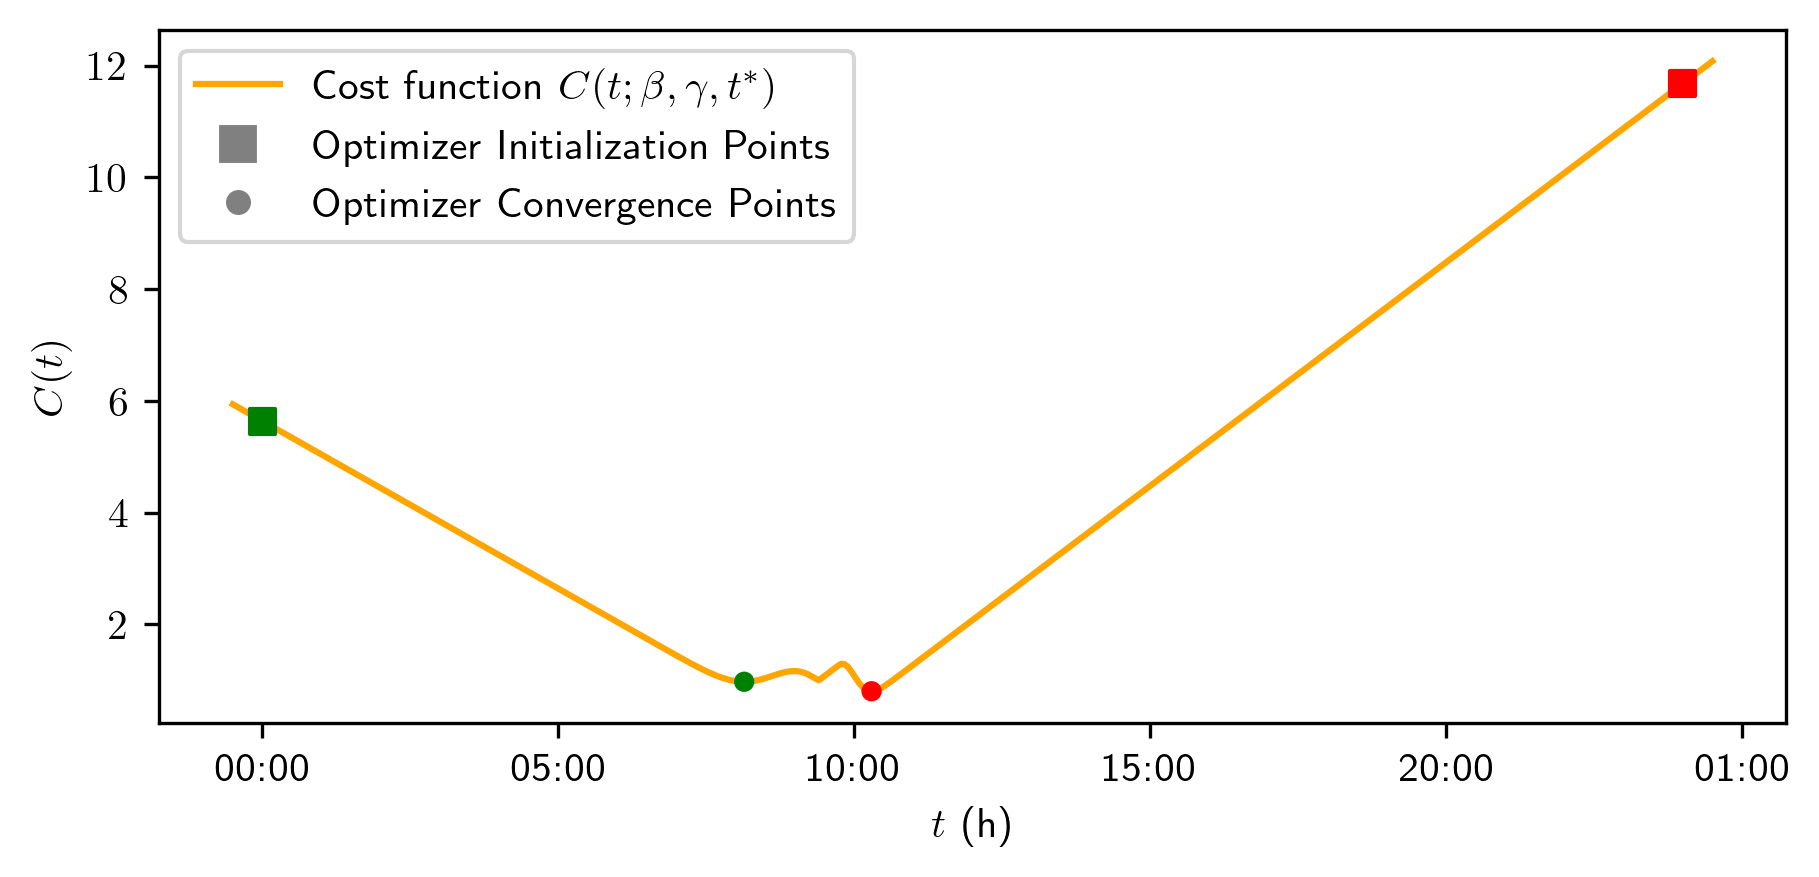
\includegraphics[width=.8\textwidth]{optimizer_cost}
  \caption{
    Cost function,
    plotted with points corresponding to the optimizers initializations and the minima at which they converge.
    The optimizer in green converges to the early minimum,
    while the one in red converges to the late minimum.
    Comparing the found minima with the cost of arriving on-time the minimizer of the cost is found.
    Parameter values used for this cost function are \(\beta = 0.6, \gamma = 0.8\).
  }
  \label{fig:optimizer-cost}
\end{figure}

Figure~\ref{fig:optimizer-cost} shows the cost function,
and depicts how the optimization process is performed.

\begin{figure}
  \centering
  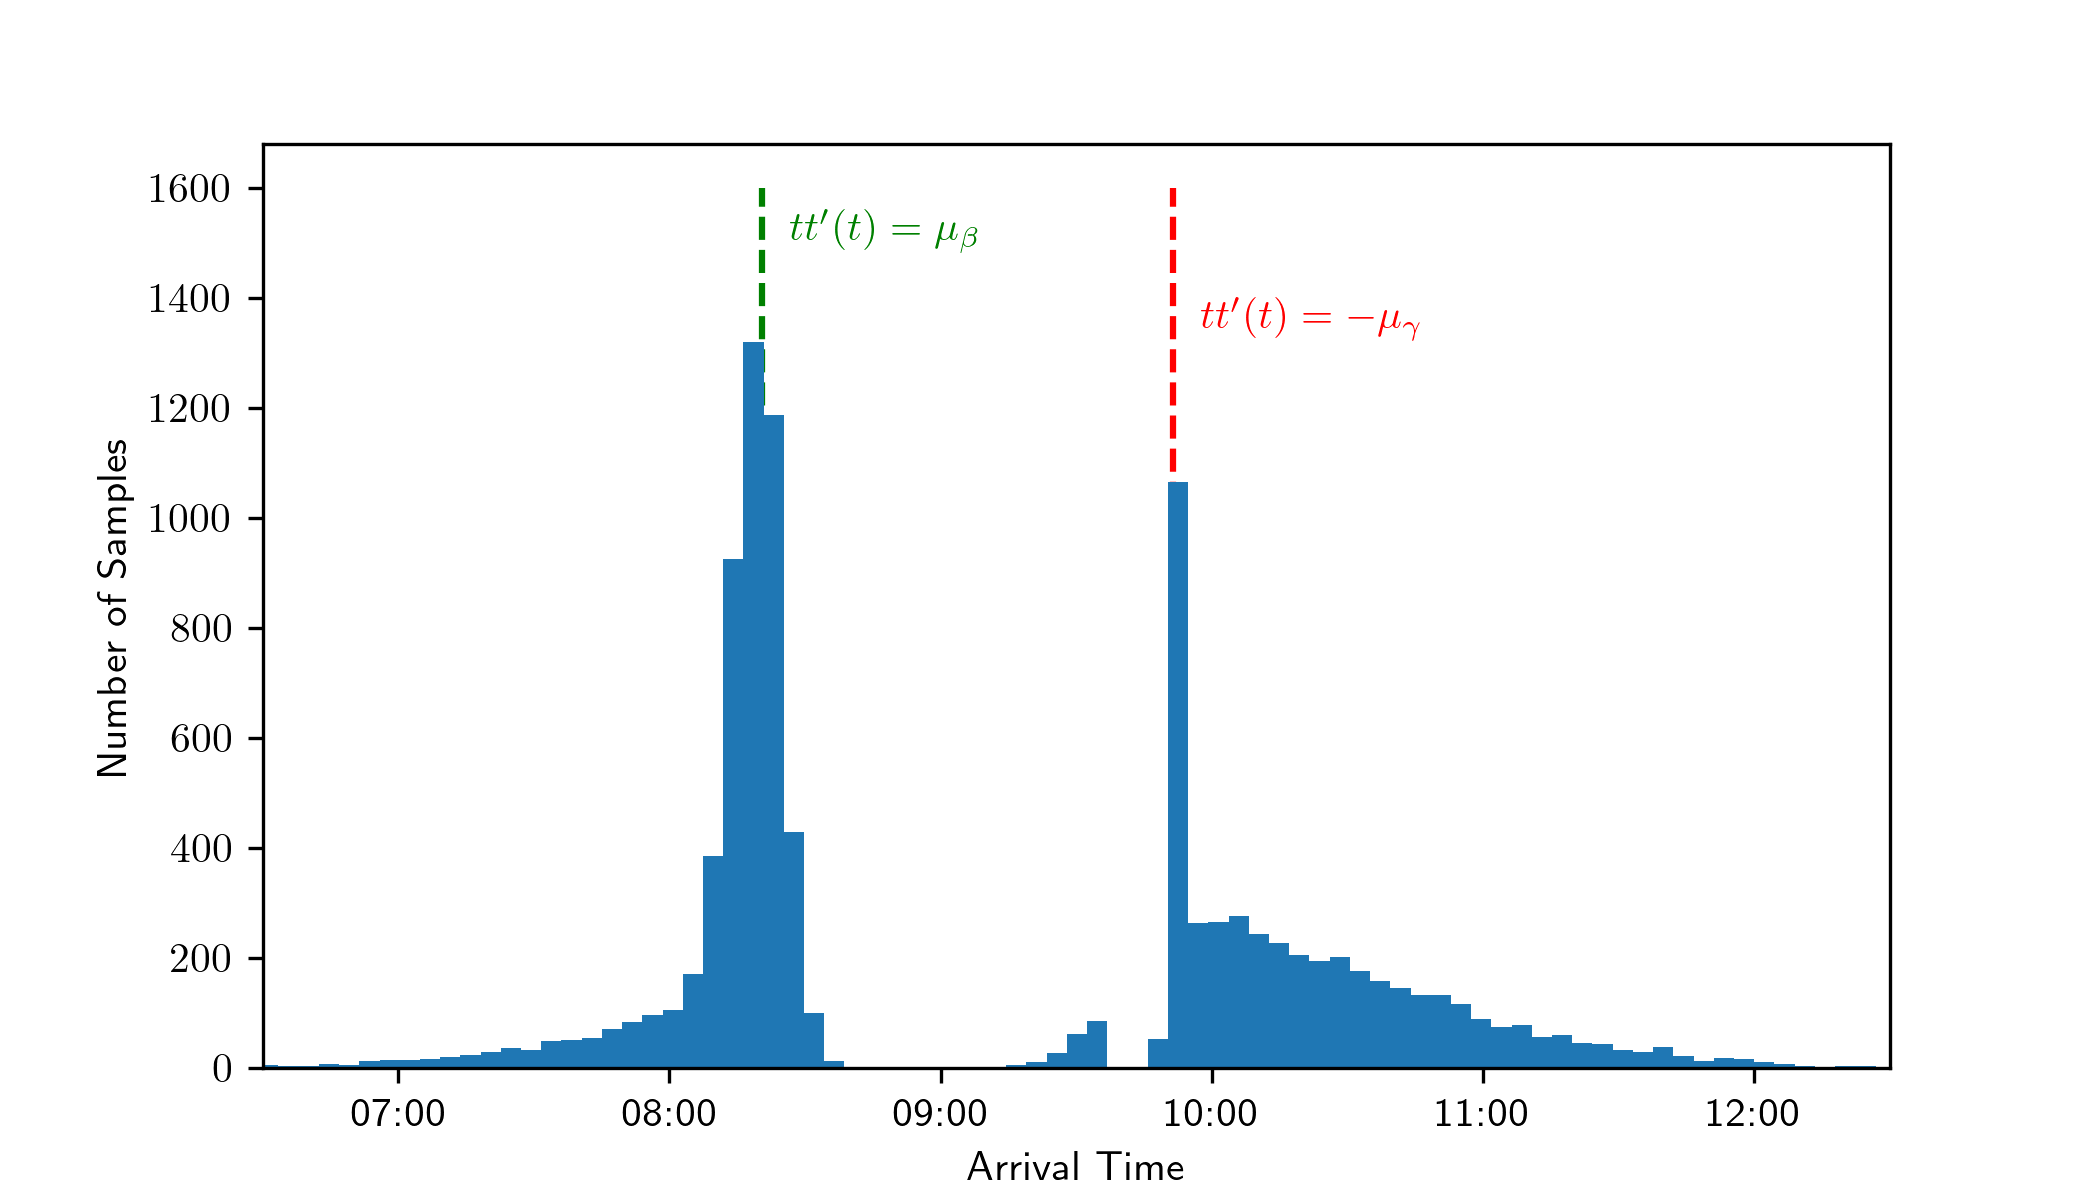
\includegraphics[width=.8\textwidth]{hist_means}
  \caption{
    Histogram displaying the distribution of \(N=10,000\) sampled arrival times,
    with parameters shown in equation~\eqref{param-hist}.
    The dashed lines show the points in which the derivative of the travel time function is equal to the scheduling delay preferences mean,
    that correspond, as expected,
    to the zones in which the density is higher.
  }
  \label{fig:hist-means}
\end{figure}

Once the minimisation process terminates,
a dataset of an arbitrary number of samples is created.
Figure~\ref{fig:hist-means} shows the result of the process,
with parameters
\begin{equation}
  \label{param-hist}
  \theta_0 =
  \begin{pmatrix}
    \mu_\beta \\
    \mu_\gamma \\
    \mu_t \\
    \sigma \\
    \sigma_t
  \end{pmatrix}
  =
  \begin{pmatrix}
    0.6 \\
    2.4 \\
    9.5 \\
    0.1 \\
    1
  \end{pmatrix}
\end{equation}

Two peaks of the arrival time density can be clearly distinguished.
The peaks correspond, as the dashed line show, to the points in which most early and late arrivals are realized
(which, according to what discussed in section \todo{put number},
occur where the derivative of the travel time function is close to the scheduling delay parameters),
and are followed (or preceded) by a zone in which the density of arrival times is particularly low,
that corresponds to the zone in which on-time arrivals are not convenient,
into the interval \todo{Specify the interval with new notation}.

\subsection{Numerical Computation of the Likelihood}

After the dataset on which the method can be performed is found,
the density of the random variable \(T^{opt}\),
as found in equation~\eqref{eq:lik-final},
must be computed.

Computing the likelihood presents some challenges,
that require modern and fast computational frameworks to be utilized.
The challenges are mostly three:
\begin{enumerate}
\item \textbf{Evaluating Critical Points}:
  the bounds for critical early (and late) arrival intervals have to be precisely estimated,
  as well as values for the coefficients \(\beta_0, \gamma_0\).
  This requires inverting the derivative of the travel time function,
  that is computationally non trivial.
\item \textbf{Estimating Integral Results}:
  as can be easily seen in equation~\eqref{eq:lik-final},
  several integrals have to be approximated.
  Doing so in a precise and fast way poses another challenge to the method
\item \textbf{Scalability}:
  the main challenge is posed by scalability;
  the likelihood of several thousands of points has to be estimated,
  and an optimization process performed on the result.
  The method must thus keep a good precision,
  while being highly scalable.
\end{enumerate}

In order to tackle the three problems together,
we employ accelerated computing frameworks, that are mainly used in Machine Learning.

Using JAX \citep{jax}, a Python library developed by Google for Machine Learning purposes,
we are able to perform a precise estimation thanks to the automatic differentiation,
while reaching high scalability thanks to the just-in-time (jit) compilation of the code.

The intervals are hence computed by utilizing iterative algorithms in JAXopt \citep{jaxopt},
that allows to just-in-time compile gradient descent and bisection algorithms,
necessary for computing the bounds of the critical intervals\todo{write something more specific here?}.

Lastly, integrals are computed using Gaussian Quadrature \citep{gauss_quad},
whose implementation in the package quadax allows, again,
just-in-time compilation and automatic differentiation of the result.

The resulting code is available at \url{github.com/something}.

Once the estimation of the density can be performed,
the parameters can be fixed to plot the density for different values of arrival time.

\begin{figure}
  \centering
  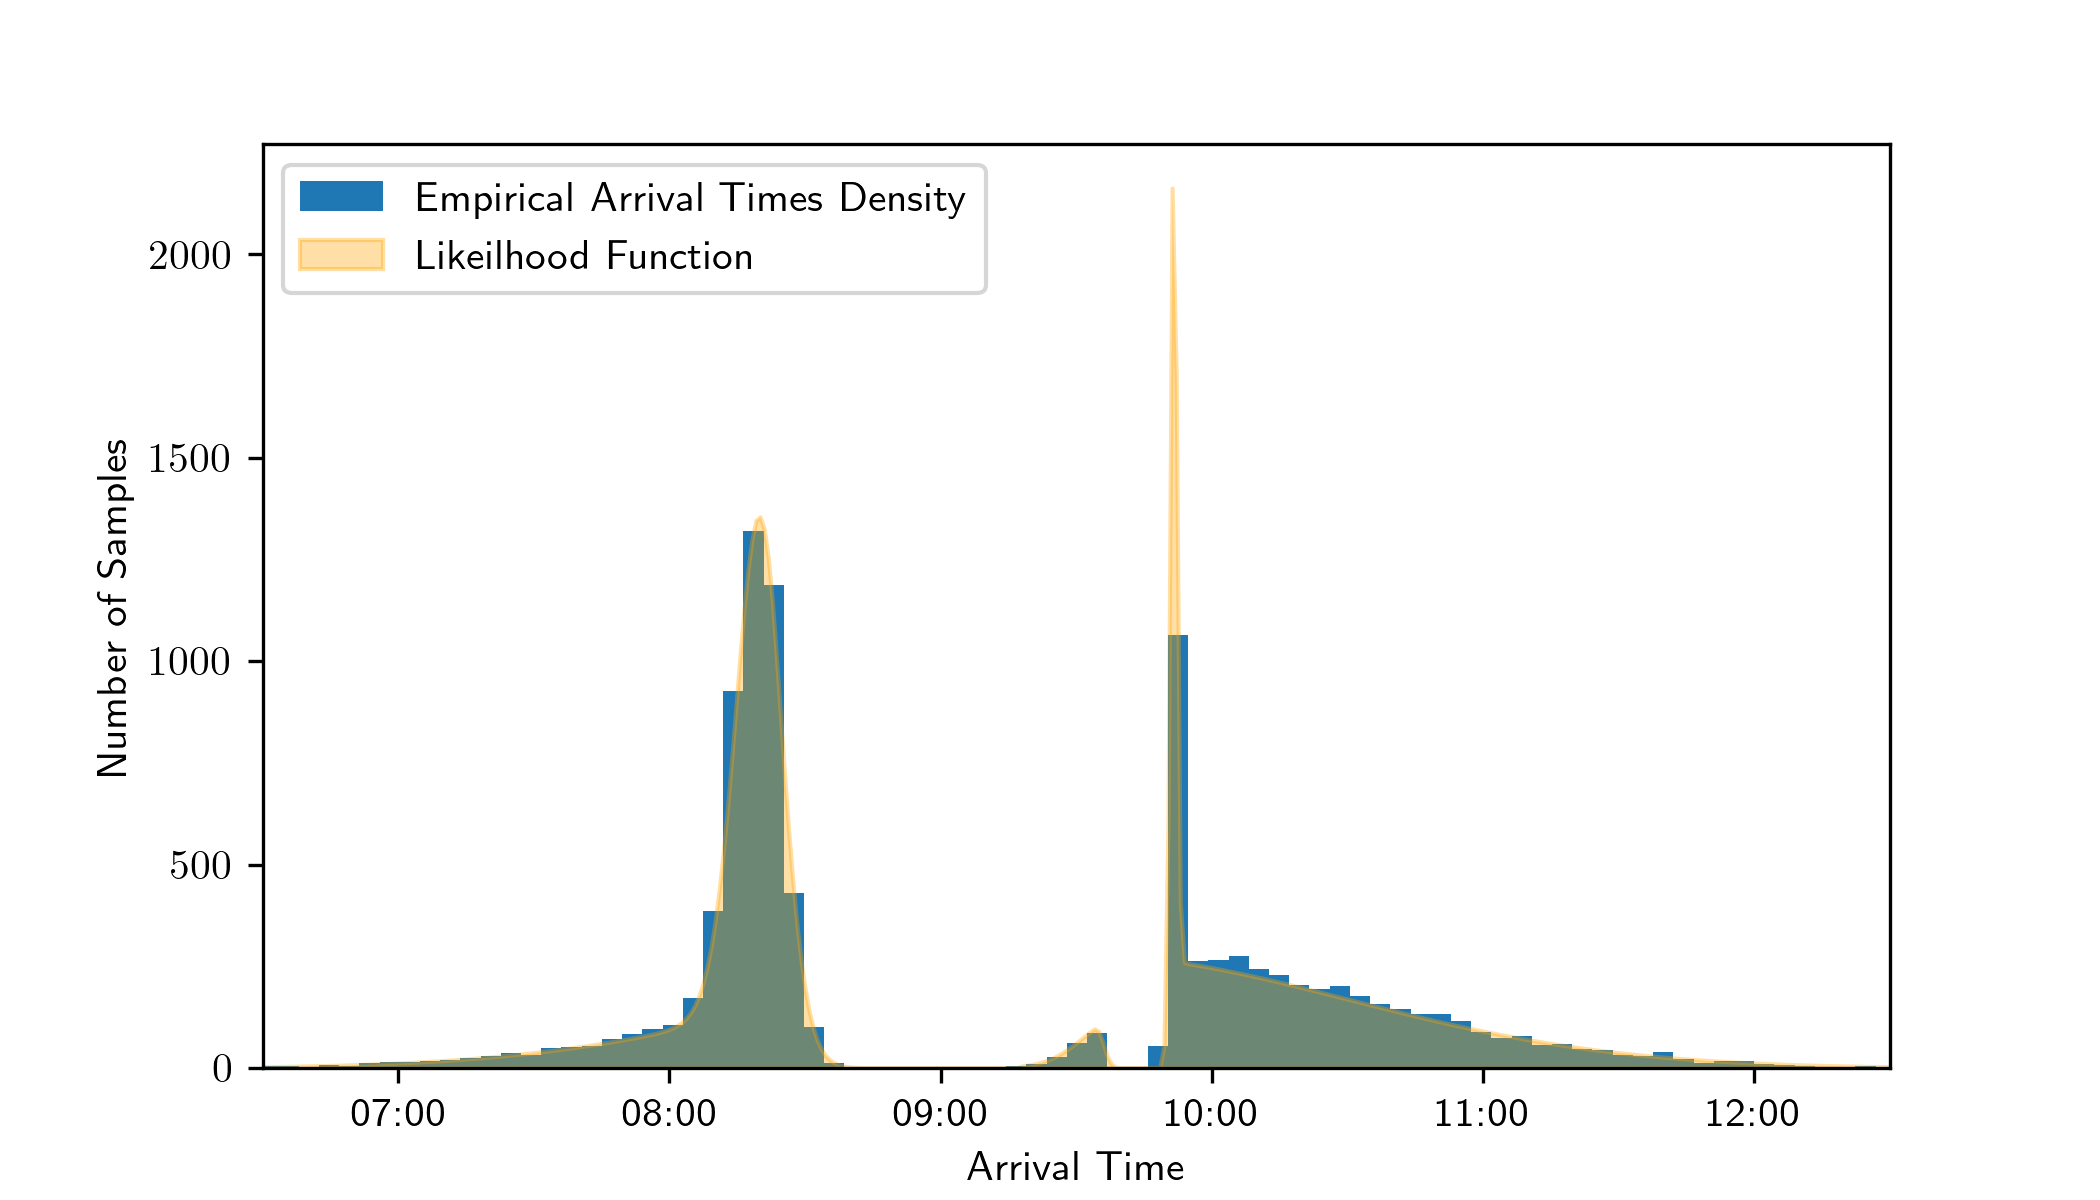
\includegraphics[width=.8\textwidth]{hist_lik}
  \caption{Histogram displaying the distribution of \(N=10,000\) sampled arrival times,
    plotted over the result of the likelihood function in expression~\eqref{eq:lik-final}.
  The empirical distribution closely follows the predicted one.}
  \label{fig:hist-lik}
\end{figure}

Figure \ref{fig:hist-lik} shows the result of this process,
plotted over the empirical density obtained by sampling as in section~\ref{sec:synthetic-dataset}.
The parameters are the same defined before, in equation~\eqref{param-hist}.

Note that the theoretical density closely follows the empirical one,
showing the precision of the theoretical study and the accuracy of the numerical methods.
The high-performance frameworks utilized allow moreover the estimation to be performed in tolerable times,
avoiding the need of particularly powerful machines.

\subsection{Optimization of the likelihood}



%%% Local Variables:
%%% mode: LaTeX
%%% TeX-master: "../main"
%%% End:
